\documentclass{beamer}
\usefonttheme{professionalfonts}
\usetheme[subsectionpage=progressbar]{metropolis}
\setbeamertemplate{section in toc}[sections numbered]
\setbeamertemplate{subsection in toc}[subsections numbered]

\title{Riemannian Symmetric Rank One Trust Region Method}
\subtitle{in \lstinline!Manopt.jl!}
\author{Tom-Christian Riemer}
\institute{TU Chemnitz}
\date{Research Seminar Numeric,\\ 9th Juny 2021}

%packages
\usepackage{amsmath}
\usepackage[british]{babel}
\usepackage[utf8]{inputenc}
\usepackage{enumerate}
\usepackage{graphicx}
\usepackage{mathtools}
\usepackage{color}
\usepackage{listings}
\usepackage[]{algorithm2e}
\usepackage{numapde-manifolds}

\lstset{basicstyle=\ttfamily,	tabsize=2}

\newcommand\myeq{\stackrel{\mathclap{\mbox{$def$}}}{=}}

\newcommand{\Pb}[1]{\expandafter\hat#1}

\begin{document}

\maketitle

\begin{frame}{Contents}
	\tableofcontents
\end{frame}

\section{Introduction}

\begin{frame}{Riemannian Optimization}
    Finding a \textbf{minimum} of a real-valued function $f$ on a Riemannian manifold, i.e.
    \begin{equation*}
        \min f(x), \quad x \in \mathcal{M}.
    \end{equation*}\\[1.\baselineskip]
    \begin{center}
        \textbf{Riemannian manifold} = smooth manifold + Riemannian metric. \\[1.\baselineskip]
    \end{center}
    \begin{equation*}
        \mathbb{S}^{n-1} = \{ x \in \mathbb{R}^n \colon \; \lVert x \rVert_2 = 1 \}
    \end{equation*}
\end{frame}

\begin{frame}{Euclidean Trust Region Method}
    Quadratic model at current iterate:
	\begin{equation*}
    	m_k(s) = f(x_k) + {\nabla f(x_k)}^{\mathrm{T}} s + \frac{1}{2} s^{\mathrm{T}} H_k s.
    \end{equation*}
	Finding a step (e.g. tCG):
	\begin{equation*}
        s_k = \arg \min_{\lVert s \rVert_2 \leq \Delta_k} m_k(s)
    \end{equation*}
	where $\Delta_k > 0$ defines the trust region. The candidate of next iterate is
	\begin{equation*}
        \tilde{x}_{k+1} = x_k + s_k.
    \end{equation*}
	If $(f(x_k) - f(\tilde{x}_{k+1}))/(m_k(0) - m_k(s_k)) > \rho$ then $x_{k+1} = \tilde{x}_{k+1}$, the model $m_k(\cdot) \rightarrow m_{k+1}(\cdot)$ and trust region $\Delta_k \rightarrow \Delta_{k+1}$ will be updated accordingly. 
\end{frame}

\begin{frame}{Riemannian Metric and Tangent Spaces}
    \vspace{-1\baselineskip}\hfill{\tiny{[Absil, Mahony, Sepulchre, 2008]}}
    \begin{center}
        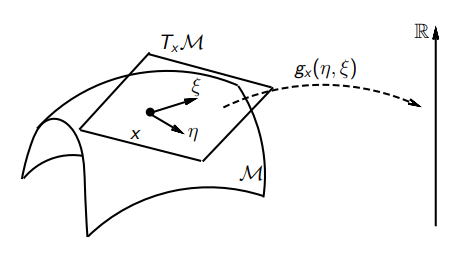
\includegraphics[width=5cm]{img/Riemannian_Metric.png}
    \end{center}
    \textbf{Tangent space} $\tangent{x}$ at $x$, with inner product $g_x(\cdot, \cdot)$. \\[0.2\baselineskip]
    \textbf{Riemannian gradient} $\mathrm{D} \, f(x) [\eta_x] = g_x (\operatorname{grad} f(x), \eta_x), \; \forall \eta_x \in \tangent{x}$. \\[0.2\baselineskip]
\end{frame}

\begin{frame}{Retractions}
    \vspace{-1\baselineskip}\hfill{\tiny{[Bergmann, 2017]}}
    \begin{center}
        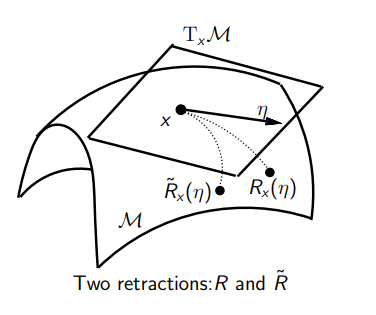
\includegraphics[width=4.5cm]{img/Retraction.png}
    \end{center}
    \textbf{Retraction} $R_{x}(\xi_x) \in \mathcal{M}$ with $R_x (0_x) = x$ and $\mathrm{D} \, R_x (0_x)[\xi_x] = \xi_x$.
\end{frame}

\begin{frame}{Quadratic Term}
	\begin{equation*}
		m_k(\eta) = f(x_k) + g_{x_k}(\operatorname{grad}f(x_k), \eta) + \frac{1}{2} g_{x_k}(\eta, \mathcal{H}_k [\eta]).
	\end{equation*}
    \textbf{Newton} TR Method: $\mathcal{H}_k = \operatorname{Hess} f(x_k) \colon \tangent{x_k} \to \tangent{x_k}, \; \eta_{x_k} \mapsto \nabla_{\eta_{x_k}} \operatorname{grad} f(x_k)$
	\textbf{SR1} TR Method: $\mathcal{H}_k \approx \operatorname{Hess} f(x_k)$
\end{frame}

\begin{frame}{Vector Transports}
    \vspace{-1\baselineskip}\hfill{\tiny{[Bergmann, 2017]}}
    \begin{center}
        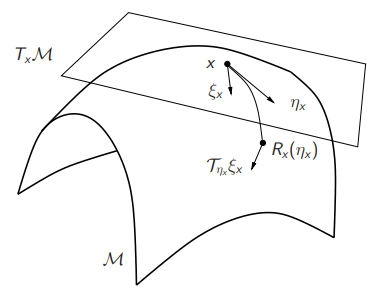
\includegraphics[width=4.5cm]{img/Vector_Transport.png}
    \end{center}
    \textbf{Isometric VT} satisfies $\lVert \nu_x \rVert_x = \lVert T^{S}_{x, \xi_x}(\nu_x) \rVert_{R_x(\xi_x)}$.
\end{frame}

\section{Numerics}

\begin{frame}{Rayleigh Quotient Minimization}
    $A \in \mathbb{R}^{n \times n}$ symmetric, the unit-norm eigenvector, $v \in \mathbb{R}^n$, corresponding to the smallest eigenvalue, defines the two global minima, $\pm v$, of the Rayleigh quotient  
    \begin{equation*}
        \begin{split}
            f \colon \; \mathbb{S}^{n-1} & \to \mathbb{R} \\
            x & \mapsto x^{\mathrm{T}} A x 
        \end{split}
    \end{equation*}   
    with its Riemannian gradient \\[.3\baselineskip]
    \begin{equation*}
        \operatorname{grad} f(x) = 2(Ax - x x^{\mathrm{T}} A x).
    \end{equation*}
\end{frame}

\begin{frame}{Experiment}
    Julia Code
\end{frame}

\begin{frame}{Results}
    Table with results.
\end{frame}

\section{Conclusion}

\begin{frame}{Conclusion}
    
    \begin{center}
        Thank you for your attention! Questions? 
    \end{center}
\end{frame}

\end{document}
